\documentclass[11pt,letterpaper]{article}
\usepackage{fontspec}
\usepackage{polyglossia}\setmainlanguage{english}
\setmainfont{TeX Gyre Termes}\setsansfont{TeX Gyre Heros}\setmonofont{TeX Gyre Cursor}
\usepackage[margin=2.4cm]{geometry}
\usepackage{amsmath,amssymb}
\usepackage{graphicx,booktabs,enumitem,xcolor,array}
\usepackage[numbers,sort&compress]{natbib}
\usepackage[font=small,labelfont=bf]{caption}
\usepackage{tikz}\usetikzlibrary{positioning,arrows.meta,fit,calc}
\usepackage{microtype}
\usepackage{lineno}
\usepackage[colorlinks=true,linkcolor=black,citecolor=black,urlcolor=blue!50!black]{hyperref}
\usepackage{authblk}
\renewcommand\Affilfont{\small}
\setlength{\parskip}{2pt}
\linenumbers

\title{\bfseries High internal accuracy, chance-level external performance: a preregistered external validation of NSGA-II electrode selection for EEG-based detection of mild cognitive impairment}
\author[1]{Jessica Milagros Cordero Rivera}
\author[1,*]{Ana Carolina Torres Villegas}
\author[1]{Salvador Miguel Hinojosa Cervantes}
\affil[1]{Tecnológico de Monterrey, Campus Guadalajara, Zapopan, Jalisco, Mexico}
\affil[*]{Corresponding author: \href{mailto:torresvillegasanacarolina@gmail.com}{torresvillegasanacarolina@gmail.com}}
\date{}

\begin{document}
\maketitle

\begin{abstract}
\noindent\textbf{Background.} A recent study reported up to 95\% accuracy in detecting mild cognitive impairment (MCI) from resting-state EEG with 5--7 electrodes selected by a multi-objective genetic algorithm (NSGA-II), using leave-one-subject-out validation in 24 people. Selection and evaluation used the same people, and no external test was performed.
\textbf{Methods.} We reconstructed the method independently and used the original public dataset (EEG\_1) only for development, where we quantified segment leakage, selection bias and ocular contamination. We froze the replication and four alternatives (ICA-cleaned relative band power with shrinkage LDA, without selection, with one electrode per scalp zone, with NSGA-II and with a penalised binary particle swarm), preregistered hypotheses, decision rules and code fingerprints on OSF, and tested every method once on an independent public dataset from the same centre and equipment (EEG\_2; 18 MCI, 16 controls). A secondary analysis used a physical montage processed channel by channel.
\textbf{Results.} In development, mixing segments of the same person raised accuracy from 50--57\% to 90--99\%, and NSGA-II reached 72--79\% with shuffled labels. Externally, the replication's internal accuracy of 75.1\% fell to a balanced accuracy of 45.8\% (95\% CI 31.2--60.1), supporting our first hypothesis. No method performed above chance ($p_\text{Holm}=1.00$); the four alternatives predicted MCI for all 34 people, so their formal non-inferiority was trivial. The two datasets were 94.4\% distinguishable from EEG features alone: EEG\_2 was dominated by delta activity (69\% against 40\% of 1--30\,Hz power), and mains interference was associated with the diagnosis in opposite directions in the two datasets. External AUCs were 0.40--0.52, and per-dataset standardisation revealed no residual signal. The physical-montage comparison was inconclusive.
\textbf{Conclusions.} The reported accuracies did not transfer to new people. Dataset shift and acquisition confounders outweighed any MCI-related signal. Electrode minimisation should follow, not precede, person-level, nested and preregistered external validation.\\[4pt]
\noindent\textbf{Keywords:} mild cognitive impairment; EEG; channel selection; NSGA-II; external validation; preregistration; replication; dataset shift.
\end{abstract}

\begin{figure}[t]
\centering\resizebox{\linewidth}{!}{%
\begin{tikzpicture}[every node/.style={font=\scriptsize, align=center},
  box/.style={draw, rounded corners=2pt, minimum height=13mm, text width=27mm, fill=#1}, box/.default=gray!8,
  arr/.style={-{Stealth[length=2mm]}, thick}]
\node[box=blue!8]   (d1)  at (0,0)     {\textbf{EEG\_1}\\24 people\\(11 MCI, 13 controls)};
\node[box]          (dev) at (3.6,0)   {\textbf{Development}\\replication\\+ diagnostic controls};
\node[box]          (frz) at (7.2,0)   {\textbf{Freeze}\\R, M0, M4, M1, M6\\+ physical montage};
\node[box=orange!12](reg) at (10.8,0)  {\textbf{Preregistration}\\hypotheses, rules,\\SHA-256 of code and data};
\node[box=blue!8]   (d2)  at (14.4,0)  {\textbf{EEG\_2}\\34 people\\(18 MCI, 16 controls)};
\node[box=orange!12, text width=52mm] (tst) at (12.6,-2.4) {\textbf{Single external test}\\fit on EEG\_1, predict EEG\_2 once;\\script applies the registered rules};
\draw[arr] (d1) -- (dev); \draw[arr] (dev) -- (frz); \draw[arr] (frz) -- (reg);
\draw[arr] (reg.south) -- (reg.south |- tst.north); \draw[arr] (d2.south) -- (d2.south |- tst.north);
\draw[dashed, gray] (12.6,1.0) -- (12.6,-0.9); \node[font=\tiny, text=gray] at (12.6,1.25) {no access before registration};
\end{tikzpicture}}
\caption{\textbf{Study design.} EEG\_1 was used for everything that involves choices; EEG\_2 was used once, after the preregistration, by frozen code.}
\label{fig:design}
\end{figure}

\section{Introduction}

Mild cognitive impairment (MCI) is a decline in cognition beyond what is expected for age that does not yet compromise independence, and it is a frequent precursor of dementia \citep{petersen2004}. Resting-state electroencephalography (EEG) is attractive for screening because it is inexpensive, non-invasive and portable, and because MCI and Alzheimer's disease are associated with a slowing of the resting rhythms, in particular a reduction of posterior alpha power \citep{babiloni2015,cassani2018}. A screening device would be more practical with few electrodes, so several studies search for the smallest montage that preserves diagnostic accuracy.

\citet{aljalal2024} addressed this question with a multi-objective genetic algorithm (NSGA-II; \citealp{deb2002}) that searched for the electrodes and features that maximise leave-one-subject-out (LOSO) accuracy while minimising the number of electrodes. Using a public dataset of 24 people from Isfahan \citep{kashefpoor2016}, they reported 89.7\% accuracy with all 19 electrodes, up to 94.9\% with 7 electrodes, and up to 95.8\% when features were also selected. The electrodes chosen most often were Cz, F8, T4 and Fp1. The code was not released.

Three well-documented pitfalls can inflate such figures. First, when segments of the same person appear in both training and test sets, a classifier can recognise the person instead of the condition \citep{saeb2017}. Second, when the same cross-validation estimate is used both to choose a model (here, the electrode subset) and to report its performance, the reported value is optimistically biased, and the bias grows with the number of candidate models \citep{varma2006,cawley2010}. NSGA-II evaluates thousands of subsets, so this selection bias can be large. Third, with a few dozen people the sampling error of any accuracy estimate is wide, about $\pm 15$ percentage points \citep{varoquaux2018}, so apparent improvements are easily produced by chance. A fourth, domain-specific issue concerns the frontal electrodes: Fp1, Fp2, F7 and F8 record eye movements, which can differ between groups and act as a confounder. Finally, electrodes selected after an average reference and an independent component analysis (ICA) computed from all 19 channels are \emph{virtual}: their signal contains information from the other electrodes, and a device with only those electrodes could not reproduce it.

The only way to know whether a selected montage generalises is to test it once on people who were never used to build or select it \citep{collins2024}. We therefore (i) reconstructed the method of \citet{aljalal2024} independently in Python; (ii) used the original dataset (EEG\_1) only for development, where we quantified the pitfalls above with diagnostic controls; (iii) froze the replication and four alternatives designed to address them; (iv) preregistered hypotheses, decision rules and code fingerprints \citep{nosek2018,osfprereg}; and (v) ran a single external test on an independent public dataset from the same centre and equipment (EEG\_2; \citealp{kashefpoor2019}). A secondary, preregistered analysis asked whether the conclusions hold with a physical montage, in which each electrode is processed on its own.

\section{Materials and methods}

\subsection{Datasets}

Both datasets are public resting-state EEG recordings from Isfahan University of Medical Sciences, acquired with the same system (19 electrodes of the 10--20 system, 256\,Hz, about 30 minutes per recording) and distributed by the same group \citep{kashefpoor2016,kashefpoor2019}. Table~\ref{tab:data} summarises them. According to the source, MCI was diagnosed with a neuropsychiatric interview based on Petersen's criteria, with Mini-Mental State Examination (MMSE) scores of 21--26 for MCI and above 26 for controls; participants were 60--77 years old and had undergone coronary angiography in the previous year. EEG\_2 was released as an extension of the same dataset; we could not verify that its inclusion criteria are identical. The original studies obtained ethical approval and informed consent as reported in their publications; the present work is a secondary analysis of de-identified public data.

\begin{table}[t]
\centering\small
\caption{\textbf{Datasets.} Both come from the same centre and recording system. Labels were read from each dataset's \texttt{states.xlsx} file.}
\label{tab:data}
\begin{tabular}{@{}lll@{}}
\toprule
 & EEG\_1 (development) & EEG\_2 (external test) \\
\midrule
People available & 27 (11 MCI, 16 controls) & 34 (18 MCI, 16 controls) \\
People used & 24 (11 MCI, 13 controls)\textsuperscript{a} & 34 (no exclusion) \\
Recording length & about 30 min & 27.3--37.9 min \\
Segments per person & 60 $\times$ 10\,s (first 10 min) & 60 $\times$ 10\,s (first 10 min) \\
Role & development and selection only & single locked test \\
Reference & \citet{kashefpoor2016} & \citet{kashefpoor2019} \\
\bottomrule
\end{tabular}

\smallskip\footnotesize\raggedright \textsuperscript{a}\,\citet{aljalal2024} excluded three controls without naming them; we excluded the three controls with the most 10-s segments above 100\,\textmu V (HC\_12, HC\_17, HC\_24). An analysis with all 27 people is reported as exploratory.
\end{table}

Before the external test we checked that no EEG\_2 recording duplicates an EEG\_1 recording: no file is identical (MD5), and the maximum correlation between any 30-s fragment of an EEG\_2 recording and any EEG\_1 recording was 0.74, against 1.00 for a true copy. All 34 EEG\_2 recordings contain the 19 channels at 256\,Hz and exceed 10 minutes.

\subsection{Independent replication of the original method}

We rebuilt the pipeline of \citet{aljalal2024} from its Methods section (Fig.~\ref{fig:design}). The first 10 minutes of each recording were band-pass filtered (0.5--64\,Hz), re-referenced to the common average, notch-filtered at 50 and 100\,Hz, and split into 60 segments of 10\,s. Each segment was decomposed with a five-level discrete wavelet transform (Daubechies-4, detail D1 discarded; \citealp{mallat1989}) or with variational mode decomposition, and ten measures were computed per sub-band and channel (among them threshold entropy, ThEn, and Teager energy, TeEng). Four classifiers (\emph{k}-nearest neighbours, support vector machine, discriminant analysis and random forest) were evaluated with LOSO, averaging the per-subject segment accuracy as in the original paper. NSGA-II used a binary chromosome over the 19 channels plus integer genes for the classifier's hyperparameters, with the two objectives of the paper: fewer channels and higher LOSO accuracy. Population and generations were 200 and 50 for channel selection. Choices that the original paper does not specify (wavelet family, ThEn threshold of 2\,\textmu V, genetic operators, z-scoring within folds, which controls to exclude) are documented in the code. Running the replication on two different computers produced identical results in all 80 measure--decomposition--classifier combinations.

\subsection{Diagnostic controls on the development data}

On EEG\_1 only, we quantified the pitfalls described in the Introduction: (i) record-wise 10-fold cross-validation, which mixes segments of the same person, versus person-wise LOSO; (ii) NSGA-II run with shuffled diagnostic labels, which shows the accuracy that the search reaches without any real signal \citep{ojala2010}; (iii) nested LOSO, in which NSGA-II selects electrodes on 23 people and the selected model is tested on the 24th, repeated 24 times \citep{varma2006}; and (iv) the ocular content of each electrode, estimated as the share of its variance explained by the ICA components most correlated with vertical and horizontal electro-oculograms derived from the frontal channels \citep{jung2000}.

\subsection{Methods compared in the external test}

Five methods were frozen in code before the preregistration (Table~\ref{tab:methods}). R is the replication of \citet{aljalal2024} in its best-reported channel-selection configuration (DWT, ThEn, discriminant analysis), with the paper's rule of keeping the solution with the highest internal accuracy. M0, M4, M1 and M6 share a cleaner representation designed to address the pitfalls: (a) ICA removal of the two components most correlated with vertical and horizontal eye movements, exclusion of Fp1, Fp2, F7 and F8 and recomputation of the average reference; (b) features that the MCI literature associates with the condition, namely the log relative power in the delta (1--4\,Hz), theta (4--8\,Hz), alpha (8--13\,Hz) and beta (13--30\,Hz) bands, computed with Welch's method \citep{welch1967} on each 10-s segment and averaged per person, so that the unit of analysis is the person and not the segment; and (c) a regularised classifier, linear discriminant analysis with Ledoit--Wolf shrinkage \citep{ledoit2004}. M0 uses the 15 remaining electrodes without selection. M4 restricts the search to one electrode per scalp zone (frontal, central, temporal, parieto-occipital; 180 combinations evaluated exhaustively), a much smaller search space that leaves fewer opportunities to fit noise. M1 applies NSGA-II with the paper's rule to the same features. M6 uses binary particle swarm optimisation \citep{kennedy1997} with an explicit penalty of one percentage point per electrode, to check that conclusions do not depend on the search algorithm \citep{wolpert1997}. For M1 and M6 the prediction for each person is the majority vote of five seeds. All selection inside M4, M1 and M6 uses an inner leave-one-out on the training people.

\begin{table}[t]
\centering\footnotesize
\caption{\textbf{Methods frozen before the external test.} All are fitted, and select their electrodes, on EEG\_1 only. LDA: linear discriminant analysis; LOO: leave-one-out.}
\label{tab:methods}
\begin{tabular}{@{}p{1.7cm}p{3.6cm}p{3.1cm}p{5.4cm}@{}}
\toprule
Method & Signal & Features & Electrode selection and decision \\
\midrule
R & 19 channels, average reference & DWT ThEn per segment & NSGA-II (200$\times$50, seed 0), highest internal LOSO accuracy; person label = majority of segments \\
M0 & ICA-cleaned, 15 channels\textsuperscript{a} & Log relative band power, person mean & None (15 electrodes); shrinkage LDA \\
M4 & As M0 & As M0 & One electrode per zone, exhaustive search (180), inner LOO balanced accuracy \\
M1 & As M0 & As M0 & NSGA-II (40$\times$25) with the paper's rule; majority vote of 5 seeds \\
M6 & As M0 & As M0 & Binary PSO (20 particles, 25 iterations), fitness = inner balanced accuracy $-$ 1 point per electrode; vote of 5 seeds \\
M0-phys., M4-phys. & 15 channels, per-channel filtering only (no average reference, no ICA) & As M0 & As M0 and M4 \\
\bottomrule
\end{tabular}

\smallskip\raggedright \textsuperscript{a}\,Fp1, Fp2, F7 and F8 removed after ICA; average reference recomputed.
\end{table}

\paragraph{Physical montage.} In M0 and M4, each electrode's features are computed after an average reference and an ICA estimated from all 19 channels. To test whether the electrode savings hold with real electrodes, M0-physical and M4-physical repeat M0 and M4 with only single-channel operations (band-pass and notch filtering), keeping the original recording reference. This analysis was added after the main methods were frozen and was preregistered as secondary.

\subsection{Preregistration and external test}

Hypotheses, decision rules, the code (SHA-256 fingerprints of every file) and the extracted EEG\_2 feature files (also fixed by SHA-256; extraction is deterministic and reproduces them bit for bit) were registered on OSF before any model was trained or evaluated on EEG\_2 \citep{osfprereg}. The external test was then run once: every method was fitted on EEG\_1 and predicted each EEG\_2 person, and a script applied the preregistered decision rules to the saved predictions.

The primary outcome was the person-level balanced accuracy on the 34 EEG\_2 people, i.e., the mean of sensitivity and specificity. The research question (RQ) asked which methods perform above chance; each method's predictions were held fixed and the test labels permuted 10\,000 times, with Holm correction across the five methods \citep{holm1979}. Four hypotheses were registered:
\begin{itemize}[leftmargin=*,itemsep=1pt]
\item \textbf{H1.} R shows high internal accuracy but much lower external accuracy. Supported if R's internal LOSO accuracy (the figure the original paper would report) lies above the upper limit of the 95\% bootstrap confidence interval (CI) of its external balanced accuracy.
\item \textbf{H2.} M0 is not inferior to R.
\item \textbf{H3.} M4 and M6 are not inferior to M1 and use fewer electrodes (median over seeds).
\item \textbf{H4 (secondary).} M0-physical is not inferior to M0 with ICA. Because M4-physical fell to 36.7\% in development (Section~\ref{sec:dev}), no prediction was made for it.
\end{itemize}
Non-inferiority \citep{walker2011} used a margin of $-10$ percentage points of balanced accuracy, the smallest loss we considered relevant for screening and about the size of the gain that artefact cleaning gave in development. It was assessed with a paired bootstrap of people stratified by class (10\,000 resamples; \citealp{efron1993}); non-inferiority was concluded if fewer than 5\% of resampled differences were at or below $-10$, i.e., if the lower limit of the two-sided 90\% CI was above $-10$. Holm correction was applied across the two comparisons of H3 and, separately, of H4. Exact Clopper--Pearson intervals \citep{clopper1934} are reported for raw accuracy. With 18 MCI and 16 controls, a method needs at least 62\% balanced accuracy to beat chance; the power to detect true balanced accuracies of 60, 70 and 80\% is 0.40, 0.84 and 0.99 (simulation). A CI containing both $-10$ and 0 is reported as inconclusive.

As a descriptive control for domain shift, a shrinkage LDA with leave-one-out tried to tell from the 15-electrode features alone which dataset each of the 58 people came from (\emph{dataset effect}).

\subsection{Exploratory analyses}

The following analyses were declared as exploratory in the preregistration: (i) the external test of M0 and M4 trained on all 27 people of EEG\_1; (ii) the area under the ROC curve (AUC), estimated with leave-pair-out in EEG\_1 \citep{airola2011} and externally for the methods with a continuous score; (iii) mains interference, measured as the log ratio of power at 49--51\,Hz to power at 1--45\,Hz in the raw recordings, and slow frontal activity (0.5--4\,Hz power at Fp1, Fp2, F7 and F8), both compared between groups and datasets; (iv) a positive control, the direction of the group difference in posterior alpha relative power (P3, Pz, P4, O1, O2), which is expected to be lower in MCI \citep{babiloni2015}; and (v) the stability of the electrodes selected by M1 and M6 across seeds.

\subsection{Software and reproducibility}

All analyses were run in Python with MNE-Python \citep{gramfort2013}, scikit-learn \citep{pedregosa2011}, NumPy and SciPy. NSGA-II and binary PSO were implemented from their original descriptions. All stochastic steps use fixed seeds. The code, the preregistration and the analysis outputs are available at the OSF registration and in the accompanying repository.

\section{Results}

\subsection{Development data (EEG\_1)}\label{sec:dev}

\paragraph{Mixing segments of the same person explains most of the reported accuracy.} With the 19 channels and person-wise LOSO, the replication reached 49.9--56.6\% (segment accuracy averaged per person) for six representative combinations, close to the 54\% of always predicting the majority class (Fig.~\ref{fig:dev}). When segments of the same person were allowed in both training and test folds (record-wise 10-fold cross-validation), the same features and classifiers reached 89.8--99.2\%. The value reported by \citet{aljalal2024} for their best all-channel combination (DWT-STD-LDA, 89.7\%) is closer to our record-wise estimate (89.8\%) than to our person-wise estimate (54.4\%).

\begin{figure}[t]
\centering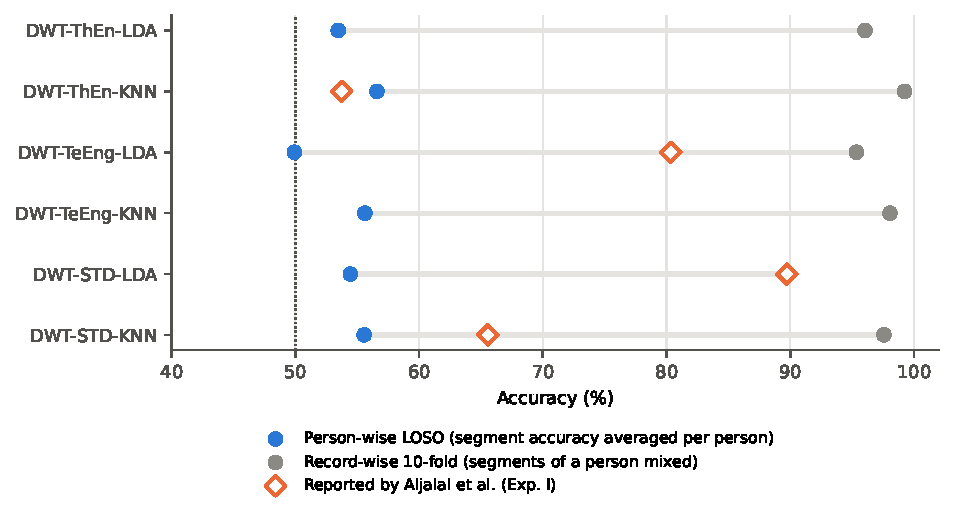
\includegraphics[width=\linewidth]{../figs/en_dev.pdf}
\caption{\textbf{Person-wise versus record-wise validation in the development data.} Same DWT features and classifiers, 19 channels, EEG\_1 (24 people). Blue: LOSO with all segments of the held-out person excluded from training. Grey: 10-fold cross-validation over segments, which mixes segments of the same person. Diamonds: all-channel values reported by \citet{aljalal2024} (Experiment I), where available. Dotted line: 50\%.}
\label{fig:dev}
\end{figure}

\paragraph{Electrode selection fits noise.} Running NSGA-II with shuffled diagnostic labels produced internal LOSO accuracies of 72--79\%, equal to or higher than those obtained with the real labels (65--75\%). In nested LOSO (DWT-ThEn-KNN), the subset chosen on 23 people reached 67\% internally but 40\% on the held-out person. With the cleaner features, the paper's selection rule obtained 48\% in nested LOSO against 61\% without selection, and with shuffled labels one method still reached 71\% under nested evaluation, which illustrates how wide the chance distribution is with 24 people.

\paragraph{Frontal electrodes carry ocular signal.} The share of variance explained by ocular ICA components was 72\% at Fp2, 68\% at Fp1, 52\% at F7 and 39\% at F8, with a clear drop for the remaining electrodes. Horizontal eye-movement activity was larger in the MCI group (uncorrected $p=0.015$; exploratory). Two of the four electrodes most often selected by \citet{aljalal2024} (Fp1 and F8) are therefore among the most contaminated.

\paragraph{Cleaner features did not produce a reliable signal.} ICA cleaning improved balanced accuracy by about 9 points across feature types (from about 48\% to 57\%; $p\approx0.14$). In nested LOSO, M0 reached 61.2\% (AUC 0.61) and M4 64.3\% (AUC 0.61), neither above chance (permutation $p=0.24$ and $0.11$). The leave-pair-out AUC of M0 was 0.65. With the physical montage M0 kept its balanced accuracy (61.2\%; AUC 0.57; leave-pair-out AUC 0.57), but M4 fell to 36.7\% (AUC 0.29) and chose a different combination in almost every fold. These results were known before the preregistration and are why H4 made no prediction for M4-physical.

\subsection{Preregistered external test (EEG\_2)}

The test was run once, after the registration was submitted, with code and feature files whose SHA-256 fingerprints matched the registered ones. Table~\ref{tab:ext} and Fig.~\ref{fig:main} give the results.

\begin{table}[t]
\centering\small
\caption{\textbf{Preregistered external test.} Every method was fitted and selected its electrodes on EEG\_1 (24 people) and was evaluated once on EEG\_2 (34 people: 18 MCI, 16 controls). Balanced accuracy with 95\% stratified bootstrap CI; permutation $p$ with Holm correction across the five main methods. AUC is given where the method produces a continuous score.}
\label{tab:ext}
\begin{tabular}{@{}lccccccc@{}}
\toprule
Method & Electrodes & Correct & Sens. (\%) & Spec. (\%) & Balanced acc. (\%) [95\% CI] & $p_\text{Holm}$ & AUC \\
\midrule
R & 5 & 15/34 & 16.7 & 75.0 & 45.8 [31.2, 60.1] & 1.00 & -- \\
M0 & 15 & 18/34 & 100 & 0 & 50.0 [50.0, 50.0] & 1.00 & 0.52 \\
M4 & 4 & 18/34 & 100 & 0 & 50.0 [50.0, 50.0] & 1.00 & 0.47 \\
M1 & 5\textsuperscript{a} & 18/34 & 100 & 0 & 50.0 [50.0, 50.0] & 1.00 & -- \\
M6 & 5\textsuperscript{a} & 18/34 & 100 & 0 & 50.0 [50.0, 50.0] & 1.00 & -- \\
\midrule
M0-physical & 15 & 18/34 & 72.2 & 31.2 & 51.7 [36.8, 67.0] & --\textsuperscript{b} & 0.44 \\
M4-physical & 4 & 15/34 & 50.0 & 37.5 & 43.8 [28.1, 61.1] & --\textsuperscript{b} & 0.40 \\
\bottomrule
\end{tabular}

\smallskip\footnotesize\raggedright \textsuperscript{a}\,Median over five seeds (range 4--5 for M6). \textsuperscript{b}\,Not part of the chance test family; uncorrected permutation $p=0.56$ and $0.86$.
\end{table}

\begin{figure}[t]
\centering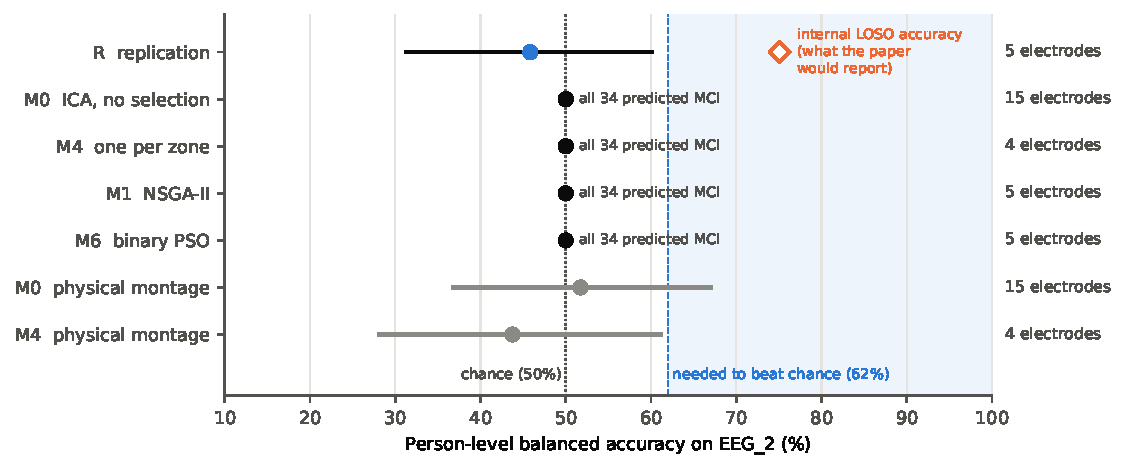
\includegraphics[width=\linewidth]{../figs/en_main.pdf}
\caption{\textbf{No method detected MCI above chance in new people.} Person-level balanced accuracy on EEG\_2 with 95\% bootstrap CI. The shaded area is the range a method needed to reach to beat chance with 34 people. The diamond is the internal LOSO accuracy of the replication on EEG\_1, the figure the original paper's procedure would report. Four methods predicted MCI for all 34 people, so their accuracy is exactly 50\% with no spread.}
\label{fig:main}
\end{figure}

\paragraph{RQ: no method beat chance.} After Holm correction no method performed above chance ($p_\text{Holm}=1.00$ for all five). The replication R classified 15 of 34 people correctly (balanced accuracy 45.8\%), with sensitivity 16.7\% and specificity 75.0\%; its segment-level accuracy was 45.6\%. M0, M4, M1 and M6 predicted MCI for every EEG\_2 person (sensitivity 100\%, specificity 0\%), a degenerate outcome explained in Section~\ref{sec:shift}.

\paragraph{H1 was supported.} On EEG\_1, NSGA-II selected T3, Cz, T4, Pz and P4 (two of them, Cz and T4, among the electrodes most often chosen by \citealp{aljalal2024}) with an internal LOSO accuracy of 75.1\%, the figure the original procedure would report. This value lies above the upper limit of the 95\% CI of the external balanced accuracy (60.1\%); the drop was 29.3 points.

\paragraph{H2 and H3 were met only trivially.} M0 was formally non-inferior to R (difference $+4.2$ points, 90\% CI $-7.6$ to $+16.0$, $p=0.026$), and M4 was formally non-inferior to M1 with fewer electrodes (4 against 5; difference 0, $p_\text{Holm}<0.001$). M6 used the same median number of electrodes as M1, so its part of H3 was not supported. Because M0, M4, M1 and M6 all predicted the same class for every person, these comparisons are uninformative: they show that a constant prediction is not worse than R or than another constant prediction, not that the cleaner or more parsimonious methods detect MCI (Fig.~\ref{fig:diff}).

\paragraph{H4 was inconclusive.} The physical montage changed balanced accuracy by $+1.7$ points for M0 (90\% CI $-10.4$ to $+14.3$; $p_\text{Holm}=0.15$) and by $-6.2$ points for M4 ($-20.5$ to $+8.3$; $p_\text{Holm}=0.31$). Both intervals include the margin and zero, so non-inferiority was not shown and inferiority was not shown either.

\begin{figure}[t]
\centering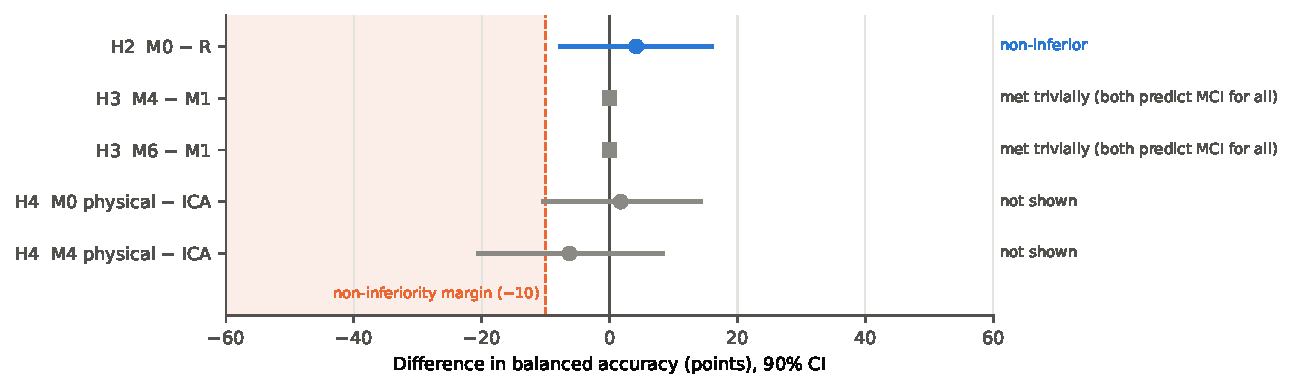
\includegraphics[width=\linewidth]{../figs/en_diff.pdf}
\caption{\textbf{Preregistered paired comparisons.} Difference in balanced accuracy on the same 34 people with 90\% paired bootstrap CI; non-inferiority required the lower limit to be above $-10$ (dashed line). Squares mark comparisons between two methods that predicted MCI for everyone, which are met trivially.}
\label{fig:diff}
\end{figure}

\subsection{Why the methods failed: dataset shift and acquisition confounders}\label{sec:shift}

\paragraph{The two datasets are almost perfectly distinguishable.} The descriptive control classified the dataset of origin of the 58 people from their 15-electrode features with 94.4\% balanced accuracy, far above the 75\% threshold we registered for a large domain shift. In EEG\_2 the delta band accounted for 68.8\% of the 1--30\,Hz power on average, against 39.7\% in EEG\_1, while alpha fell from 21.7\% to 8.0\% (Fig.~\ref{fig:conf}, left). In EEG\_1 the MCI group had more delta than controls (43.5\% against 36.4\%), so every model learned that more delta means MCI; applied to EEG\_2, where everyone has more delta than anyone in EEG\_1, they assigned all 34 people to MCI. Within EEG\_2 the direction was reversed (67.1\% in MCI against 70.7\% in controls).

\begin{figure}[t]
\centering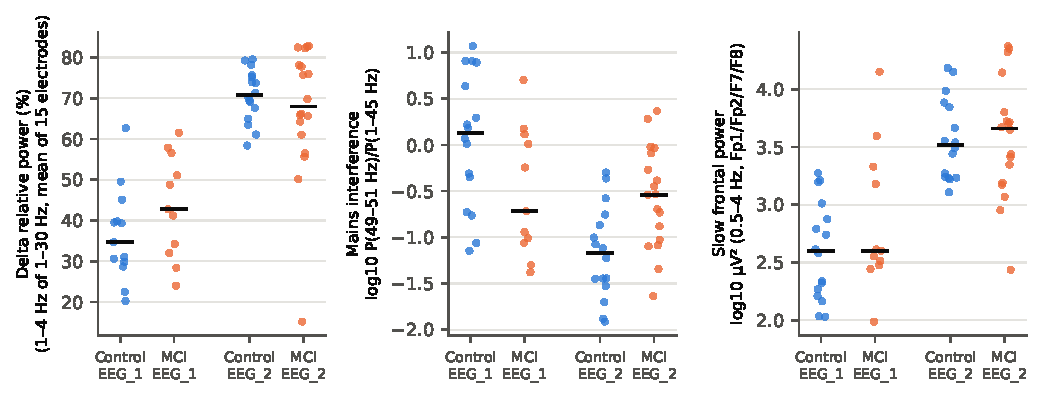
\includegraphics[width=\linewidth]{../figs/en_conf.pdf}
\caption{\textbf{Differences between datasets are larger than differences between groups.} Each dot is a person; bars are medians. Left: delta relative power, the feature that drives the classifiers. Middle: mains interference in the raw recordings; its association with the diagnosis reverses between datasets. Right: slow frontal power, about nine times higher in EEG\_2.}
\label{fig:conf}
\end{figure}

\paragraph{Mains interference is associated with the label, in opposite directions.} The relative power at 49--51\,Hz in the raw recordings differed between datasets ($p<0.001$) and was associated with the diagnosis in both, but in opposite directions: in EEG\_1 controls had more interference than MCI (AUC 0.28 for interference as a predictor of MCI; $p=0.064$), whereas in EEG\_2 MCI had more interference than controls (AUC 0.79; $p=0.004$). Acquisition conditions are thus entangled with the diagnostic groups in a way that does not transfer between datasets.

\paragraph{Model scores track slow frontal activity.} Slow frontal power (0.5--4\,Hz at Fp1, Fp2, F7 and F8) was about nine times higher in EEG\_2 ($p<0.001$) and did not differ between groups within either dataset. In EEG\_2, the continuous score of M0 correlated with this frontal slow power (Spearman $\rho=0.42$, $p=0.012$) and not significantly with the diagnosis (AUC 0.52), even though the frontal electrodes had been removed and ocular components subtracted.

\subsection{Exploratory analyses}

\paragraph{No ranking signal either.} The AUC, which does not depend on the decision threshold and is therefore insensitive to a global shift, was 0.52 for M0, 0.47 for M4, 0.44 for M0-physical and 0.40 for M4-physical. Training on all 27 people of EEG\_1 did not change the picture (AUC 0.41--0.54). In a post hoc analysis that was not preregistered, standardising each dataset with its own mean and standard deviation (without labels) removed the global shift but did not reveal a signal: AUC 0.52 for M0 ($p=0.44$) and 0.45 for M4 with ICA, 0.42 and 0.38 with the physical montage.

\paragraph{The positive control pointed in the expected direction but was weak.} Posterior alpha relative power was lower in MCI than in controls in both datasets, as expected \citep{babiloni2015}, but the effect was small and not significant (AUC 0.59, $p=0.49$ in EEG\_1; 0.57, $p=0.48$ in EEG\_2; similar with the physical montage).

\paragraph{Selected electrodes were stable but not valid.} M1 chose the same subset (F4, T4, T5, Pz, T6) with four of five seeds, and M6 chose T4 and T6 with all five seeds and F4 and Pz with four (Fig.~\ref{fig:heads}). This stability across seeds did not translate into external performance.

\begin{figure}[t]
\centering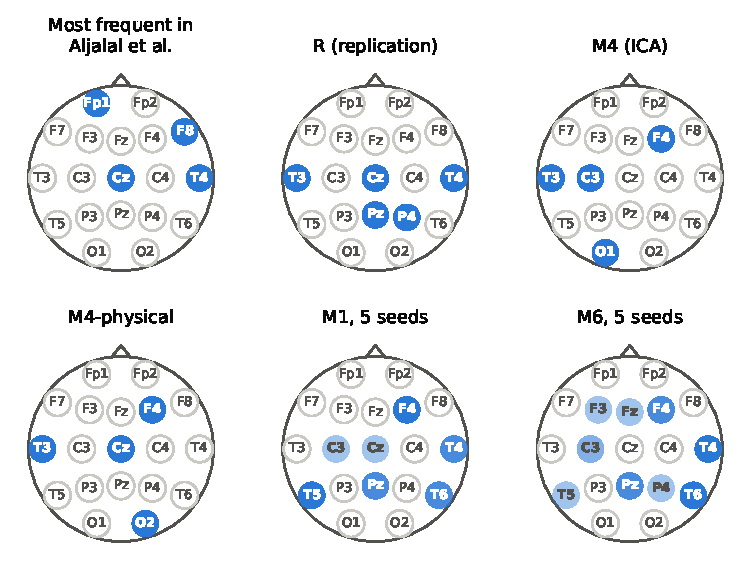
\includegraphics[width=0.82\linewidth]{../figs/en_heads.pdf}
\caption{\textbf{Electrodes selected on EEG\_1.} Darker means selected more often (across seeds for M1 and M6). Fp1 and F8, two of the electrodes most often selected by \citet{aljalal2024}, are among the most contaminated by eye movements; M0--M6 exclude Fp1, Fp2, F7 and F8 by design.}
\label{fig:heads}
\end{figure}

\section{Discussion}

In a preregistered external test, an independent replication of NSGA-II electrode selection for MCI detection reached 75.1\% internal accuracy with five electrodes and 45.8\% balanced accuracy in 34 people it had never seen. Four alternatives built to avoid the known pitfalls did not do better: all of them classified every new person as MCI. No method, with any number of electrodes and with either montage, detected MCI above chance in the new cohort.

\paragraph{Where the published accuracies come from.} Three mechanisms, each measured in the development data, can account for the gap between the published accuracies and our results. First, when segments of the same person are used for training and testing, accuracies of 90--99\% are reached with features that give chance-level results when people are kept separate; the all-channel figure reported by \citet{aljalal2024} is closer to the former. We cannot tell from the paper how the folds were built, so this is a compatibility statement, not a claim about their code. Second, NSGA-II reaches 72--79\% internal accuracy with shuffled labels, so an internal accuracy of 75\% after selection carries no evidence of diagnostic value; nested evaluation and external testing remove this bias \citep{varma2006,cawley2010}. Third, two of the most frequently selected electrodes (Fp1 and F8) are dominated by ocular signal. These mechanisms do not require any error in the original analysis: they are the expected behaviour of an unconstrained search evaluated on the same 24 people, which is why we addressed them by design and by testing on new people.

\paragraph{Dataset shift dominates.} The most informative finding was not planned as a hypothesis: two public datasets from the same centre and recording system are 94\% separable from their EEG alone, and the difference (a delta-dominated spectrum in EEG\_2, nine times more slow frontal power and a different mains interference profile) is larger than any difference between MCI and controls. We cannot determine its cause from the released files; vigilance, electrode impedance, filtering or recording period are possible explanations. Its consequence, however, is clear: a model that has learned a small group difference in delta power will move the whole new cohort across its decision boundary. Per-dataset standardisation removed the global shift but revealed no residual signal, so the failure is not only a calibration problem. The opposite association of mains interference with the diagnosis in the two datasets shows that acquisition conditions can be confounded with the groups. In such small datasets any method that searches widely, whether it optimises electrodes, features or classifiers, is likely to find these confounders.

\paragraph{What the cleaner methods did and did not achieve.} The alternatives were designed to remove three sources of optimism: segment leakage, selection bias and ocular contamination. They succeeded in the sense that their internal estimates were honest (around 61--64\% in nested LOSO, never above chance), but they did not create a signal that does not exist in these data. The formal confirmations of H2 and H3 are therefore not evidence that they work; they only show that their failure was no worse than that of the original method. Parsimonious selection was at least not harmful, and the electrodes selected by NSGA-II and PSO were stable across seeds. Stability, however, did not imply validity: a stable subset can be stably fitted to a confounder.

\paragraph{Virtual versus physical electrodes.} Electrode-minimisation studies usually compute each channel after average referencing and ICA over the full montage, and then report the selected channels as if a device could use them alone. The physical montage tests this directly. In development, the one-per-zone method lost most of its accuracy with physical electrodes; externally, the comparison was inconclusive because neither montage worked. We recommend that future studies report both versions.

\paragraph{Recommendations.} Based on these results we suggest the following minimum protocol for studies that select EEG electrodes for diagnosis: evaluate by person, never by segment; keep selection inside the validation loop (nested); compare against the same procedure run on shuffled labels; report AUC as well as accuracy; check whether the selected electrodes are contaminated by eye movements and whether acquisition variables (such as mains interference) differ between groups; report a physical-montage version; test whether datasets can be told apart before pooling or transferring them; and preregister a single external test \citep{nosek2018,collins2024}.

\paragraph{Limitations.} The sample sizes are small, so the external test could only detect large effects (power 0.84 for a true balanced accuracy of 70\%) and the non-confirmed hypotheses are inconclusive rather than negative. EEG\_2 was released as an extension of the same dataset, but we could not verify that its diagnostic and inclusion criteria, recording protocol or period are identical, and the cause of the dataset shift remains unknown. Our replication rests on documented assumptions where the original paper is not specific (wavelet family, entropy threshold, genetic operators, which controls were excluded), and the external test covered the paper's best channel-selection configuration (DWT, ThEn, discriminant analysis), not every feature combination or the joint feature selection of its Experiment III. Only the first 10 minutes of each recording were analysed, no age or sex information was available, and the ICA component rule was automatic. Some development diagnostics (shuffled labels, ocular contamination) were computed before this registration and are reported as development results. Finally, the per-dataset standardisation was post hoc. None of these limitations favours the conclusion that the original accuracies transfer: each would, if anything, make a transferable signal easier to find.

\section{Conclusions}

The high accuracies reported for NSGA-II electrode selection in MCI detection from resting EEG did not survive an independent, preregistered external test: internal accuracy of 75\% became 46\% in new people, and none of four cleaner or more parsimonious alternatives performed above chance. The decisive factor was a large shift between two datasets from the same centre, together with acquisition variables associated with the diagnostic groups. Minimising electrodes is only meaningful once a signal has been shown to generalise; until then, we recommend person-level, nested and externally validated evaluation, with physical montages and preregistered analyses.


\section*{Preregistration}
Hypotheses, decision rules, code and test-feature fingerprints were registered on OSF before the external test: \url{https://osf.io/4enh8}. Deviations: none in the confirmatory analysis. The per-dataset standardisation in the exploratory analyses was added after seeing the results and is labelled post hoc.

\section*{Data availability}
Both datasets are publicly available from Isfahan University of Medical Sciences at \url{https://misp.mui.ac.ir/en/eeg-data} \citep{kashefpoor2016,kashefpoor2019}. The extracted feature files can be regenerated bit for bit with the released code; their SHA-256 fingerprints are listed in the preregistration.

\section*{Code availability}
The full code (replication, frozen methods, physical montage, decision rules, exploratory analyses and figures) is available in the OSF registration and in the accompanying public repository.

\section*{Ethics statement}
This is a secondary analysis of de-identified, publicly available data. The original studies obtained ethical approval and informed consent as reported in their publications \citep{kashefpoor2016,kashefpoor2019}.

\section*{Author contributions}
\textbf{J.M.C.R.}: conceptualisation, methodology, software, investigation, formal analysis, writing -- original draft. \textbf{A.C.T.V.}: conceptualisation, methodology, software, validation, formal analysis, visualisation, writing -- original draft, writing -- review and editing. \textbf{S.M.H.C.}: supervision, writing -- review and editing. All authors approved the final manuscript.

\section*{Funding}
This research received no specific funding.

\section*{Competing interests}
The authors declare no competing interests.

\bibliographystyle{unsrtnat}
\bibliography{../shared/refs}

\end{document}
